%% Erläuterungen zu den Befehlen erfolgen unter
%% diesem Beispiel.
\documentclass{scrartcl}
\usepackage[utf8]{inputenc}
\usepackage[T1]{fontenc}
\usepackage[ngerman]{babel}
\usepackage{amsmath}
\usepackage{listings}
\usepackage{eurosym}
\usepackage{graphics}
\usepackage{latexsym}

\title{Projekt Dokumentation}
\author{Benjamin Franzke, Jan Klemkow und Maik Rungberg}
\date{03. Januar 2010}

\begin{document}

\maketitle
\tableofcontents

\newpage

\section{Einleitung} %% TODO
	Diese Projekt-Dokumentation beschreibt die komplette Durchfürung des Mikroprozessortechnik-Projektes,
	den Aufbau der einzelnen Schaltungen und einige technische Erläuterungen.

	In den folgenden Kapiteln werden die zwei Schaltungen und zusätzliche Entwicklungen und Umbauten erläutert.
	Als Fahrzeugschaltung wird die Schaltung bezeichnet die in das Fahrzeug verbaut wurde.
	Die Steuerschaltung ist am Computer angeschlossen und sendet die Steuerinformationen an die Fahrzeugschaltung.

\section{Umbau am Auto} %% TODO
	Als Grundlage wurde ein Funkferngesteuertes Auto (RC-Car) benutzt,
	welches im Internet bei ebay.de bestellt wurde.
	Die vorhandene Elektronik zur Funkfernsteuerung wurde entfernt
	und durch eine selbstentwickelte Fahrzeugschaltung ersetzt.
	Vom Fahrzeug wurde das Gestell, die Elektromotoren zum Antrieb und zur Lenkung,
	sowie der Akkumulator übernommen.
	An die Kabel der Elektromotoren wurden Verlängerungen gelötet,
	welche sich einfacher auf dem verwendeten Steckbrett befestigen ließen.

\newpage

\section{Fahrzeugschaltung} %% TODO
	Die Fahrzeugschaltung besteht im Wesentlichen aus einem Mikrocontroller "ATMEGA 16" und einem Funkemfänger "RFM12".
	Versorgt wird die gesamte Schaltung über die im Fahrzeug integrierte Versorungsspannung,
	welche aus einem 10 Volt Akkumulator besteht.
	Da der "ATMEGA 16" eine Spannungsversorgung von 5 Volt benötigt, ist der Festspannungsregler "L7805"
	zwischen Akkumulator und Mikrocontroller geschaltet.

	\subsection{Motoransteuerung}
		Für die Ansteuerung der Elektromotoren des Antriebs und der Lenkung sind vier Motortreiber, vom Typ "L298", verbaut.
		Diese sind aus zwei Gründen notwendig. Zum einen ist das die Steuerung der Drehrichtung der Motoren, praktisch
		bedeutet das vorwärts/rückwärts fahren respektive links/rechts.
		Des weiteren sind die Treiber notwending um den -für den Microcontroller- zu hohen Strom und die höhere Spannung
		für die Motoren zu regulieren bzw. auszuhalten.

		%% TODO: Schaltbild des L298? kann ja gefragt sein in prüfung

		Die verwendeten Bauelemente, vom typ "L298", enthalten jeweils zwei Motortreiber, welche 2A aushalten.
		Insgesamt werden zwei Bauelemente und damit vier Motortreiber benutzt.
		Drei Motortreiber sind für den Antriebsmotor parallel zusammen geschaltet, da dieser 
		bei Messungen teilweise 4A verbraucht hat, somit kann er nun maximal 6A Strom ziehen.
		Der Lenkungsmotor benötigte nur 0.5A somit sollten 2A für diesen ausreichen.
				
		%% TODO: Hier ein Bild vom internen Aufbau des Motortreibers einbinden.

		%% TODO: PWM text prüfen
		Die Geschwindigkeitsregelung ist mittels Pulsweitenmodulation im Mikrocontroller implementiert.
		Die Pulsweitenmodulation basiert auf dem Wechseln zweier Spannungswerte in kurzen Zeitabständen, wobei
		der Mittelwert der Spannungswerte verrechnet mit der Dauer des Auftreten des jeweiligen Wertes,
		der resultierenden Spannung entspricht.
		PWM ist ein DA-Wandler bei dem die Genauigkeit eine untergeordnete Rolle spielt, welche bei
		einem Motor keine Rolle spielt.

		Der Vorteil dieser Methode ist, dass nur ein Pin am ATMEGA verwerndet werden muss, und dass der ATMEGA16 die PWM
		bereits hardwareseitig implementiert hat. Dadurch fällt unnötige Rechenzeit weg.
		Die Anwendung einer solchen PWM besteht also aus der Konfiguration eines Timers,
		der hardwareseitig eine Zahl hochzählt. Dabei ist vor dem Erreichen einer bestimmten
		(eingestellbaren) Zahl der PWM-Ausgang auf Low gesetzt und danach auf High.
		So entstehen unterschiedliche lange Impulse - das arithmetische Mittel variiert je nach eingestellter Zahl.
		Daraus folgt, dass die eingestellte Zahl den Spannungswert repräsentiert.

		Am Motortreiber wird das PWM-Signal am enable Eingang angelegt, da so nur ein Timer für den Motor anfällt.
		In welche Richtung sich der Motor drehen soll, wird dann an den IN 1..4 Eingängen eingestellt.
		
	
	\subsection{Sensoren}
		Dieser Abschnitt beschreibt die Sensoren, sowie deren Funktionsweisen und Aufgaben
		in der Fahrzeugschaltung.


		\subsubsection{Lichtsensor (LDR) - Fotowiderstand} %% TODO: maik!

			Um bei Dunkelheit das Licht am Auto anzuschalten, wird ein Fotowiderstand genutzt.
			Der Fotowiderstand ändert seinen Widerstand in Abhängigkeit vom Umgebungslicht.
			Da man den Widerstand nicht direkt auslesen kann, setzt man ihn in Verbindung mit einem zweiten,
			bekannten Widerstand, als Spannungsteiler ein, und misst die hier entstehende Spannung.
			Sobald das Licht der Umgebung abnimmt, und unter einen bestimmten Wert sinkt,
			schaltet der Controller das Licht vorne am Auto an.
			So eine ähnliche Funktion bieten viele neue PKW's.

			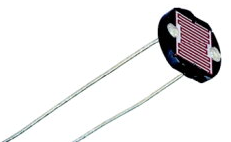
\includegraphics{images/helligkeitssensor.png}

		\subsubsection{Infrarot Abstandssensor} %% TODO: maik!
			Der Abstandssensor soll verhindern, dass das Fahrzeug frontal gegen ein Hindernis fährt.

			Sharp GP2Y0A21YK:\\
			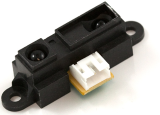
\includegraphics{images/infrarotsensor.png}

			Der Infrarot Abstandssensor von Sharp bietet eine garantierte Abstandserkennung von 10cm bis 80cm.
			In diesem Bereich liegt am Signalausgangspin (Vo) vom Sensor eine Spannung von 3.1V bis 0.4V an.
			Wie auf dem Diagramm 1 zu sehen, fällt die Spannung nach ca. 5cm stark ab
			und der Abstand zum Objekt ist aufgrund doppelter Werte nicht mehr eindeutig Zuordnungsbar. 

			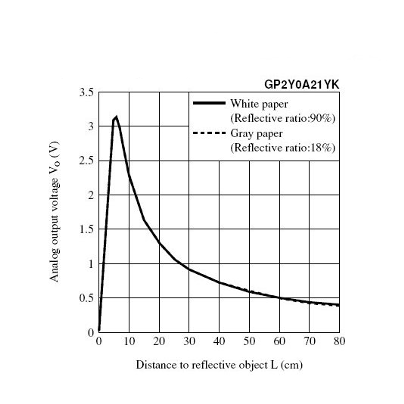
\includegraphics{images/sensordiagramm.png}

			Da der Abstandssensor aber in erster Linie dazu verwendet wird,
			weiter entfernte Objekte zu erkennen und rechtzeitig zu bremsen spielen Distanzen unter 30cm keine Rolle.
			Um mit der internen Referenzspannung, von 2.56V, des Atmega16 arbeiten zu können,
			wurde der Sensor über einen geeigneten Spannungsteiler „gedrosselt“ um die maximale Spannung nicht zu überschreiten. 

			Im Mikrocontroller arbeitet ein 8-Bit Timer mit aktivierten Vorteiler von 256.
			Zusammen mit dem internen Takt von 1Mhz findet alle ca. 66ms ein Überlauf statt.
			Die Routine für den Timerüberlauf-Interrupt wird genutzt,
			um genau nach diesen 66ms eine Messung (4 Messung des ADC's mit Bildung des arithmetischen Mittels)
			des Sensors durchzuführen und im Falle eines Objektes in Reichweite, zu bremsen.
			Da laut Datenblatt alle 38.3ms $\pm$ 9,6ms neue Werte am Ausgang anliegen, ist man auf der sicheren Seite. 

			Sobald ein Objekt innerhalb der eingestellten Reichweite vor dem Auto erscheint,
			blockiert der Controller die Vorwärtsfahrt (Rückwärts geht weiterhin)
			und zusätzlich leuchtet eine rote LED als Signal.

	
	\subsection{Programmierung} %% TODO: Erläuterung der Programmierung der Fahrzeugschaltung
		In diesem Abschnitt wird der Programmcode des Steuerkontrolers erklärt.

\newpage

\section{Steuerschaltung}

	\subsection{Kommuniation mit dem Computer} %% TODO
		Die Kommunikation zwischen Steuerschaltung und Computer findet über die RS-232-Schnittstelle statt.
		Diese Schnittstelle verwendet einen Spannungspegel von -15 bis -3 Volt zur Abbildung einer Logischen Eins 
		und einen Spannungspegel von 3 bis 15 Volt für eine Null.
		Der Bereich von -3 bis 3 Volt ist undefiniert.
		Auf Senderseite ist es üblich eine 12 Volt bzw. -12 Volt Spannungspegel für die Kommunikation zu benutzten.

		Diese Definition der RS-232 Schnittstelle, ist für den Verwendeten Mikrocontroller ein Problem,
		da dieser an seinen Pins nur eine Spannungspegel von 0 bis 5 Volt erzeugen kann.

		Zur Erzeugung des notwendigen Spannungspegels von -12 bzw. 12 Volt wird in der Steuerschaltung der Pegelwandler MAX232 benutzt.
		Die folgende Abbildung zeigt die Beschaltung des MAX-232 mit dem Mikrocontroller und der RS-232-Schnittstelle des Computers.
		%% TODO: Bild einfügen von MAX232-µC-PC

		Für die Kommunikation wird eine externer Quarz benötigt, da der intere Quarz zu ungenau und zu fehleranfällig ist.
		Bei einem Versuch mit dem internen Quarz konnte eine Kommunikation mit 600 Baud realisiert werden.
		Diese funktionierte bei einem weiteren Versuch an einem anderen Standort nicht mehr.
		Diese Phänomen kann auf die Fehleranfälligkeit, z.B. in folge von Temperaturveränderungeni, zurückgeführt werden.

	\subsection{Anbindung des Gamepad} %% TODO
		Ein Gamepad wird für die Schnittstelle zum Benutzer verwendet.
		Dafür wurde das Programm "joystick.c" in der Programmiersprache C implementiert,
		welches die Steuerinformationen vom Gamepad über die RS-232 Schnittstelle zum Steuercontroller weiterleitet.
	
	\subsection{Programmierung}
		Die Programmierung der Steuerschaltung bestand im wesentlichen in der Nutzung der hardwareseitigen UART-Implementation.
		Weiterhin wurde das Checksum verfahren genutzt um übertragungsfehler zu vermeiden.
		Das versenden selbst wird im Kapitel des Funkmoduls näher erleutert.
\newpage
\section{Funkstrecke zwischen Fahzeug- und Steuerschaltung}
	\subsection{Auswahl des Funkmoduls}
		Als Funkmodul wurde der RFM12 der Firma HOPE RF gewählt.
		Dieses Modul beinhaltet den eigentlichen Funkchip RF12 und die nötige Grundbeschaltung für die Nutzung.

		Die Gründe für die Wahl dieses Moduls liegen im günstigen Preis von 5 EURO pro Stück.
		Weiterhin bietet jedes der Module die Möglichkeit zu Senden und zu Empfangen.
		Dieses Feature wird zwar momentan nicht benutzt, aber bei weiterentwicklungen wenn man Sensordaten
		an den PC zurück schicken möchte, wird es sicher nützlich sein.
		
		Das letzte Kriterium war die einfache ansteuerbarkeit mit einem Protokoll, dass bereits im ATMEGA 
		hardwareseitig implementiert ist.
	\subsection{Implementierung}
		Das Funkmodul RF12 besitzt mehrere unterschiedliche Interfaces 
		zur Kommunikation mit dem Mikrocontroller.
		Alle Einstellungen zur Funküberragung werden Kommandobasiert
		über die SPI-Schnittstelle gesendet.

		Für das Senden/Empfangen der Daten stehen zusätzlich andere Datenleitungen
		zur Verfügung, es besteht aber auch die Möglichkeit die Daten in Befehle
		kodiert über die SPI-Schnittstelle an das Modul zu transferrieren bzw
		durch Kommandos ein Auslesen des FIFO`s zu initiieren.

		Gewählt wurde für dieses Projekt das SPI-Interface, da so die komplette 
		Kommunikation hardwareseitig ablaufen kann und so die Modul-Steuerung einheitlich ist.

		Der RF12 besitzt ein 16bit FIFO in das die Daten direkt hineingeschrieben werden können,
		Der Chip liest die Daten dann aus dem FIFO und versendet sie.
		Dies ist von Vorteil gegenüber anderen Chips des gleichen herstellers (RF02), bei dem
		musste jedes Bit einzeln Übertragen und das Versenden abgewartet werden.

	\subsection{Ablauf Senden/Empfangen}
		Der Sender schreibt zuerst eine sogenannte PREAMBLE bestehend aus dreimal 
		hintereinander 0xAA (hex). Diese signalisiert dem sendenden dass neue Daten 
		Versendet werden sollen.
		Danach wird ein Synchronisierungspattern gesendet 0x2DD4 (hex), dieser wird
		auf Empfaengerseite genutzt um sich zu synchronisieren und schlusszufolgern,
		dass Daten nun gesendet werden. Ob die Empfaengerseite einen
		Synchronisierungspattern nutzen soll ist einstellbar, eine weitere Möglichkeit
		wäre ein VDI (Valid Data Indicator). Es wurde sich in diesem Projekt
		aber für ersteres entschieden.

		Sind nun beide Funk-Chips bereit zu Senden bzw zu empfangen werden nun die Daten
		selbst an den Sender geschickt und auf Empfängerseite vom Chip gelesen.

		Beendet wird ein Transfer auf Senderseite wiederrum durch die PREAMBLE.

		Auf Empfängerseite wird ein Interrupt ausgelöst sobald 8-Bit emfpangen worden sind.
		Dieser wird mittels externem Hardware Interrupt am Microcontroller registriert.
		Sodass der Microcontroller das auslesen aus dem Funkmodul beginnt.

	\subsection{Probleme}
		Während der Entwicklung gab es immer wieder Probleme mit undokumentierten Eigentschaften,
		z.b. dass der Chip beim Starten (vom Hersteller auch POR Power-On Reset genannt)
		eine Zeit zum initialisieren brauch, diese Eigenschaften mussten aus dem Beispielcode 
		entnommen werden.
		
		Weiterhin ist das SPI-Interface teilweise verbuggt, sodass Befehle redundant verschickt 
		werden mussten.
		
		Beispiel:
		Auf Empfängerseite wird ein Interrupt ausgelöst, danach sollten nun Daten transferriert werden.
		Der Microntroller könnte also einfach den Befehl - der im Datenblatt steht - zum Auslesen des FIFO`s
		an das Funkmodul senden, doch das reicht nicht, zusätzlich musste vorher ein sogenannter
		"Status Read Command" gesendet werden, der 24-bit zurückliefert. Die ersten 16bit sind
		Statusinformationen die letzten 8-bit die Daten.
		Der Lesebefehl schickt seine Daten auf den letzten 8-bit. 
		Die Daten werden also zeimal hintereinander ausgelesen.
		
		Alles in allem sind die Funk-Ergebnisse und die Reichweite des Moduls aber so überzeugnend, dass
		diese Schwachpunkte zu verkraften sind.

\newpage

\section{Quelltext}
	In diesem Kapitel werden die einzelnen Quelltexte, der für dieses Projekt entwickelten Programme, aufgelistet.

\lstset{language=C}
\include{sources}

\end{document}

%% vim: set spelllang=de sts=0 fenc=utf-8: 
